	    % Corregir redacción, plural y presente
	
	    % TODO
	    % - Arquitectura sistemas NLG (3 slides aprox)
	    % - Requerimientos. Aca presentar la clase de prueba generada por Fastest y comentar algunas de las tranformaciones que le tendremos que hacer para generar mejores descripciones.
	    % - Desarrollo, ya con todos los requerimientos presentados, deberían ser unas pocas slides (3 o 4) por etapa.
	    %
	    % 0) Hacer algo con los exampleblock (o usarlos para todos los esquemas Z o no usarlo para ninguno). En caso de usarlos, ver la forma que queden más "lindos", que no ocupen el 100% de la página en una lista de items por ej. Multiple columns para clase y caso de prueba del ejemplo?
	    % 1) Armar un bosquejo de las slides que faltan y luego pegarle una corregida agregando todas las notas necesarias.
	    %
	
	    % Copyright 2004 by Till Tantau <tantau@users.sourceforge.net>.
	    %
	    % In principle, this file can be redistributed and/or modified under
	    % the terms of the GNU Public License, version 2.
	    %
	    % However, this file is supposed to be a template to be modified
	    % for your own needs. For this reason, if you use this file as a
	    % template and not specifically distribute it as part of a another
	    % package/program, I grant the extra permission to freely copy and
	    % modify this file as you see fit and even to delete this copyright
	    % notice. 
	
	    \documentclass{beamer}
	    \usepackage[spanish]{babel}
	    \usepackage[utf8]{inputenc}
	    \usepackage{czt}
	
	    %\usetheme{Madrid}
	    \usetheme{Antibes}
	
	    %\title{Generación de lenguaje natural a partir de clases de prueba del \textit{test template framework}}
	
	    % A subtitle is optional and this may be deleted
	    %\subtitle{Optional Subtitle}
	
	    %\author{F.~Author\inst{1} \and S.~Another\inst{2}}
	    % - Give the names in the same order as the appear in the paper.
	    % - Use the \inst{?} command only if the authors have different
	    %   affiliation.
	
	    %\institute[Universities of Somewhere and Elsewhere] % (optional, but mostly needed)
	    %{
	    %  \inst{1}%
	    %  Department of Computer Science\\
	    %  University of Somewhere
	    %  \and
	    %  \inst{2}%
	    %  Department of Theoretical Philosophy\\
	    %  University of Elsewhere}
	    % - Use the \inst command only if there are several affiliations.
	    % - Keep it simple, no one is interested in your street address.
	
	    %\date{Conference Name, 2013}
	    % - Either use conference name or its abbreviation.
	    % - Not really informative to the audience, more for people (including
	    %   yourself) who are reading the slides online
	
	    \subject{Computer Science}
	    % This is only inserted into the PDF information catalog. Can be left
	    % out. 
	
	    % If you have a file called "university-logo-filename.xxx", where xxx
	    % is a graphic format that can be processed by latex or pdflatex,
	    % resp., then you can add a logo as follows:
	
	    \pgfdeclareimage[height=0.5cm]{university-logo}{../img/unr.png}
	    \logo{\pgfuseimage{university-logo}}
	
	    % Delete this, if you do not want the table of contents to pop up at
	    % the beginning of each subsection:
	    \AtBeginSubsection[]
	    {
	        \begin{frame}<beamer>{Outline}
	            \tableofcontents[currentsection,currentsubsection]
	        \end{frame}
	    }
	
	    % Let's get started
	    \begin{document}
	
\title[NLG a partir de clases de prueba del TTF]{Generación de lenguaje natural a partir de clases de prueba del \textit{test template framework}}
\institute[FCEIA - UNR]{
  Departamento de Ciencias de la Computación\\
  Facultad de Ciencias Exactas, Ingeniería y Agrimestoy considerando en pedirme un día de estudio jueves o viernesensura\\
  Universidad Nacional de Rosario
}
\author[Julian De Tomasi]{\begin{tabular}{r@{ }l} 
  Autor:      & Julian De Tomasi \\[1ex]
  Directores: & Maximiliano Cristiá\\
  & Brian Plüss
  \end{tabular}}
\date{Marzo, 2016}
	
\begin{frame}
  \titlepage
\end{frame}
	
\begin{frame}{Outline}
  \tableofcontents
  % You might wish to add the option [pausesections]
\end{frame}
	
\section{Introducción}
	
\begin{frame}{Motivación}{}
  \begin{itemize}
            							
    \item {
        Las metodologías de \emph{testing} basado en modelos parten de un modelo formal (o especificación) del software a testear y a partir del mismo son generados los casos de prueba. 
      }
                  										
      \note[item]{
        Es una de las técnicas de testing más prometedoras para la verificación de software crítico.\\
      }
                  										
      \item {
          El TTF (\emph{Test Template Framework}) es un caso particular del testing basado en modelos. Utiliza como modelo de entrada una especificación formal en notación Z y establece cómo generar \emph{casos de prueba} para las operaciones incluidas en la especificación.
                             				  				  					      
        }
                        													
        \note[item]{
          El TTF propone en primera instancia obtener casos de prueba abstractos a partir de una especificación llamados \emph{clases de prueba} y luego, a partir de los mismos, generar los \emph{casos de prueba concretos}.\\
        }
                        													
        \item {
            Usualmente también se realizan procesos independientes de validación y verificación, llevados a cabo por expertos en el dominio que generalmente no poseen conocimiento técnico para comprender lo que se esta siendo testeado.
          }
                              																
          \note[item]{
            En estos casos, una descripción en lenguaje natural de cada caso de prueba debería acompañar a los mismos a fin de hacerlos accesibles para los expertos en el dominio.\\
          }
                              																
        \end{itemize}
      \end{frame}
                  										
                  										
      \begin{frame}{Ejemplo: SymbolTable}{Especificación}
        \begin{itemize}
          \item{La operación \emph{LookUpOk} (parte de la especificación para una tabla de símbolos) modela la búsqueda de información asociada a un símbolo perteneciente a la tabla.
          }
        \end{itemize}
                        													
        \note[item]{
          Una tabla de símbolos es una estructura de datos utilizada por un compilador o intérprete durante el proceso de traducción de un lenguaje de programación donde cada símbolo en el código del programa (variables, constantes, funciones, etc.) se asocia con información como la ubicación, tipo de datos, \textit{scope} de variables, etc. En general, en una tabla de símbolos se realizan dos operaciones: inserción/actualización y búsqueda.
        }
                        													
        \vspace{-1.0cm}
        \begin{schema}{LookUpOk}
          \Xi ST \\
          s?: SYM \\
          v!: VAL \\
          rep!: REPORT
          \where
          s? \in \dom st \\
          v! = st~s? \\
          rep! = ok
        \end{schema}
                        													
        \note[item]{
          El tipo básico \emph{SYM} representará el conjunto de todos los símbolos aceptados por el compilador/interprete, mientras que \emph{VAL} abstraerá el conjunto de toda la información que pudiese estar asociada a un símbolo.
        }
                        													
        \note[item]{
          Finalmente, resulta natural pensar que la tabla de símbolos establece una relación funcional entre los símbolos aceptados y la información asociada a cada uno de ellos.
        }
                        													
                        													
                        													
      \end{frame}
                  										
      \begin{frame}{Ejemplo: SymbolTable}{Designaciones}
                        													
        \note[item]{
          Vinculamos los términos del modelo formal a elementos relacionados con el dominio de aplicación mediante las designaciones.
        }
                        													
        \note[item]{
          Las designaciones sirven en primera instancia cuando se empieza a escribir la especificación para diferenciar un fenómeno en particular y darle un nombre. Luego, le será de utilidad al programador a la hora de leer la especificación.
        }
                        													
        \note[item]{
          Para nosotros las designaciones resultarán la principal fuente de conocimiento para nuestro sistema de NLG. Y serán fundamentales para que éste pueda generar descripciones independientes del dominio de aplicación.
        }
                        													
        \begin{itemize}
          \item{
            Utilizaremos a las designaciones de una manera similar a la propuesta por Jackson. Además del proposito habitual de las mismas, resultarán una fuente de conocimiento para nuestro sistema de NLG.
          }
                              																
          \item{
            Dentro de las designaciones que acompañan a la especificación, podemos tener las siguientes: \\
            \begin{exampleblock}{}
              \vspace{-.5cm}
              \begin{align*} 
                  & \text{Símbolo a actualizar}                      &   & \approx &   &   & s?      \\
                  & \text{Conjunto de símbolos cargados en la tabla} &   & \approx &   &   & \dom st 
              \end{align*}
            \end{exampleblock}
          }
        \end{itemize}
                        													
        \note[item]{
          Los sistemas de generación de lenguaje natural generalmente utilizan un diccionario de palabras o frases, las cuales se utilizan para referirse a fenómenos del dominio. En nuestro caso, el dominio de aplicación dependerá de la especificación en cuestión y de lo que se modele con la misma, por lo tanto, las designaciones resultarán nuestra única fuente de textos dependientes del dominio y es por eso que serán un elemento fundamental para nuestro sistema de NLG.
        }
                        													
      \end{frame}
                  										
      \begin{frame}{Ejemplo: SymbolTable}{Caso de prueba para \emph{LookUp}}
        \begin{itemize}
          \vspace{-.5cm}
          \item{
            Caso de prueba para \emph{Update\_SP\_4}:\\
            \vspace{-.5cm}
            \begin{schema}{LookUp\_ SP\_ 1\_ TCASE}\\
              LookUp\_ SP\_ 1 
              \where
              st = \{ ( sym0 , val0 ) \} \\
              s? = sym0
            \end{schema}
          }
        \end{itemize}
      \end{frame}
                  										
      \begin{frame}{Ejemplo: SymbolTable}{Clase de prueba para \emph{LookUp}}
        \begin{itemize}
          \item{
            Clase de prueba generada por medio del TTF para \emph{LookUp}:\\
            \vspace{-.5cm}
            \begin{schema}{LookUp\_ SP\_ 1}\\
              st : SYM \pfun VAL \\
              s? : SYM 
              \where
              s? \in \dom st \\
              \dom st = \{ s? \}
            \end{schema}
          }
                              																
          \item{
            Las \emph{clases de prueba} son las que contienen la información referente a las alternativas funcionales que se intentan testear mediante cada \emph{caso de prueba} generado.
          }
                              																    	
          \note[item]{
            La clase de prueba presentada es una versión simplificada de la generada por Fastest. Más adelante veremos la clase de prueba generada por la herramienta y como nuestro sistema trabajará con ella para obtener una similar a la anterior.
          }
        \end{itemize}
      \end{frame}
                  										
      \begin{frame}{Ejemplo: SymbolTable}{Descripción para \emph{Update\_SP\_4}}
                        													
        \begin{itemize}
          \item{
            Descripción en lenguaje natural para \emph{Update\_SP\_4}:\\
            \begin{exampleblock}{Se intenta actualizar un símbolo en la tabla, cuando:}
              %\begin{itemize}[leftmargin=*]
              $-$ El símbolo a actualizar es el único símbolo cargado en la tabla de símbolos.
              %\end{itemize}
            \end{exampleblock}
          }
          \item En sistemas en los que hay una gran cantidad de casos de prueba, traducir manualmente los mismos podría introducir errores humanos, reduciendo la calidad de las descripciones además de incrementar el costo del testing.
        \end{itemize}
      \end{frame}
                  										
      \begin{frame}{Objetivo general}{}
        \begin{itemize}
          \item El objetivo de este trabajo, será entonces, desarrollar una solución para la generación automática de descripciones para los casos de prueba generados por el TTF. Para esto, utilizaremos técnicas de \emph{generación de lenguaje natural}.
          \item Trabajaremos principalmente con las \emph{clases de prueba}, ya que estas son las que contienen la información referente a las alternativas funcionales que se intentan testear mediante cada \emph{caso de prueba}.
          \item Pretendemos una solución independiente del número de operaciones del modelo así como del dominio de aplicación del mismo. Para esto, junto con la utilización de técnicas de NLG, haremos uso de la información contenida en las designaciones.
        \end{itemize}
      \end{frame}
                  										
      \section{Requerimientos}
      \begin{frame}{Corpus}{Introducción}
        \begin{itemize}
          \item Reiter y Dale proponen la construcción de un corpus objetivo para extraer los requerimientos de un sistema NLG.
          \item Un corpus no es más que una colección de ejemplos de entrada y las respectivas salidas que se esperan de nuestro sistema de NLG. 
          \item Para consutruir el corpus que utilizamos en este trabajo, describimos manualmente un conjunto de clases de pruebas generados con Fastest para distintas especificaciones. Buscamos cubrir todo el rango de textos que esperamos que nuestro sistema sea capaz de producir.
            %\item En base al corpus, se extrajeron requerimientos fundamentales que sustentan una gran parte de las decisiones presentadas a lo largo del trabajo.
        \end{itemize}
      \end{frame}
                  										
      \begin{frame}{Corpus}{Requerimientos más relevantes}
        \begin{itemize}
          \item Determinamos la estructura que deberán tener las descripciones de cada clase de prueba en el texto final.
          \item Se detectaron tareas de razonamiento con los datos, como la reducción de expresiones y eliminación de tautologías. Fundamentales para la tarea de determinación de contenido.
          \item Se analizó la verbalización de expresiones y el rol de las designaciones en esta tarea. Fundamental para lexicalización.
          \item Se determinaron aspectos gramaticales que nuestro sistema de NLG debió contemplar. Necesario para la tarea de realización lingüística.
        \end{itemize}
      \end{frame}
                  										
      \section{Desarrollo}
                  										
      \subsection{Document Planning}
                  										
      \begin{frame}{Document Planner}{}
        \begin{itemize}
          \item Es el primer módulo del pipeline de nuestro sistema.
          \item Es el encargado de que el documento final tenga toda la información requerida por el usuario y que la misma se encuentre estructurada de una forma relativamente coherente.
          \item Este módulo será el ecargado de que se lleven a cabo las tareas de \textit{determinación de contenido} y \textit{estructuración del documento}
        \end{itemize}
      \end{frame}
                  										
      %\begin{frame}{Entrada y salida}{}
      %    \begin{itemize}
      %        \item TODO Imagen
      %    \end{itemize}
      %\end{frame}
                  										
      \begin{frame}{Determinación de contenido}{}
        \begin{itemize}
          \item Esta tarea involucra uno o más procesos de selección y razonamiento con los datos.
          \item La tarea de selección debe, básicamante, buscar e incluir en el \textit{document plan} la o las clases de prueba a describir.
          \item Las tareas de \textit{razonamiento con los datos} como la eliminación de tautologías y la reducción de expresiones mejoran sustancialmente la calidad de los textos generados por nuestro sistema.
        \end{itemize}
      \end{frame}
                  										
      \begin{frame}{Razonamiento con los datos}{Eliminación de tautologías}
        Esta tarea será la encargada de filtrar expresiones que no añaden información adicional a nuestras descripciones.
        \begin{figure}[H]
          \centering
          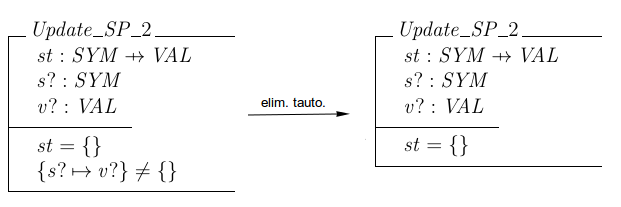
\includegraphics[scale=0.4]{img/ej_elim_tauto.png}
        \end{figure}
      \end{frame}
                  										
      \begin{frame}{Determinación de contenido}{Razonamiento con los datos}
        Esta tarea será la encargada de reducir algunas expresiones presentes en las clases de prueba geeneradas por Fastest. Permitiendo de esta forma simplificar la descripción de las mismas.
        \begin{figure}[H]
          \centering
          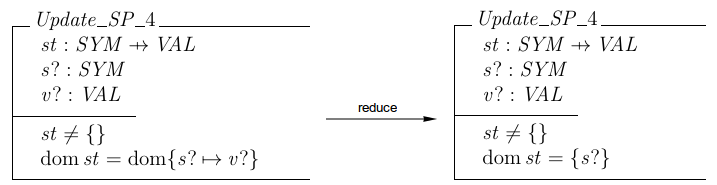
\includegraphics[scale=0.4]{img/ej_reduce.png}
        \end{figure}
      \end{frame}
                  										
      \begin{frame}{Estructuración del documento}{}
        Esta tarea será la encargada de organizar y estructurar la información que el sistema debe comunicar.
        \begin{figure}[H]
          \centering
          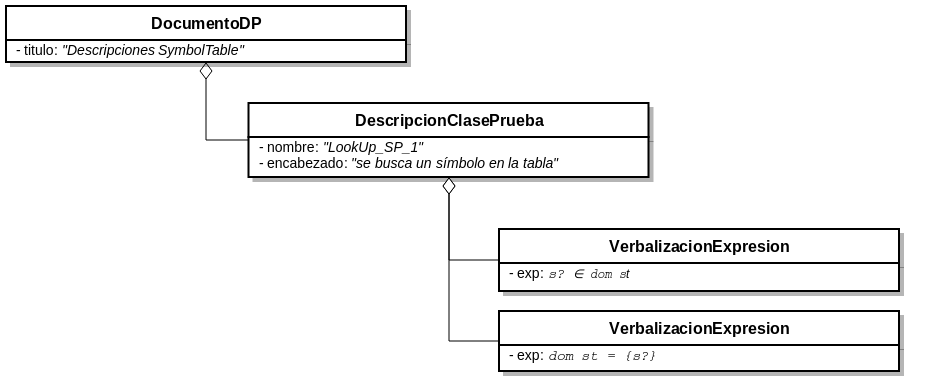
\includegraphics[scale=0.3]{img/document_plan_ej.png}
        \end{figure}
      \end{frame}
                  										
      \subsection{Microplanning}
      \begin{frame}{Entrada y salida}{}
        \begin{itemize}
          \item TODO Imagen
        \end{itemize}
      \end{frame}
                  										
      \begin{frame}{Lexicalización}{}
        \begin{itemize}
          \item TODO
        \end{itemize}
      \end{frame}
                  										
      \section{Conclusión y trabajos futuros}
      \begin{frame}{TODO}{}
                        													
      \end{frame}
                  										
      % Section and subsections will appear in the presentation overview
      % and table of contents.
      \section{First Main Section}
                  										
      \subsection{First Subsection}
                  										
      \begin{frame}{First Slide Title}{Optional Subtitle}
        \begin{itemize}
          \item {
              My first point.
            }
            \item {
                My second point.
              }
            \end{itemize}
          \end{frame}
                              																
          \subsection{Second Subsection}
                              																
          % You can reveal the parts of a slide one at a time
          % with the \pause command:
          \begin{frame}{Second Slide Title}
            \begin{itemize}
              \item {
                  First item.
                  \pause % The slide will pause after showing the first item
                }
                \item {   
                    Second item.
                  }
                  % You can also specify when the content should appear
                  % by using <n->:
                  \item<3-> {
                    Third item.
                  }
                  \item<4-> {
                    Fourth item.
                  }
                  % or you can use the \uncover command to reveal general
                  % content (not just \items):
                  \item<5-> {
                    Fifth item. \uncover<6->{Extra text in the fifth item.}
                  }
                \end{itemize}
              \end{frame}
                                          																						
              \section{Second Main Section}
                                          																						
              \subsection{Another Subsection}
                                          																						
              \begin{frame}{Blocks}
                \begin{block}{Block Title}
                  You can also highlight sections of your presentation in a block, with it's own title
                \end{block}
                \begin{theorem}
                  There are separate environments for theorems, examples, definitions and proofs.
                \end{theorem}
                \begin{example}
                  Here is an example of an example block.
                \end{example}
                \begin{beamercolorbox}[wd=7cm]{eecks}
                  asdasdasdsad
                \end{beamercolorbox}
              \end{frame}
                                          																						
              % Placing a * after \section means it will not show in the
              % outline or table of contents.
              \section*{Summary}
                                          																						
              \begin{frame}{Summary}
                \begin{itemize}
                  \item
                    The \alert{first main message} of your talk in one or two lines.
                  \item
                    The \alert{second main message} of your talk in one or two lines.
                  \item
                    Perhaps a \alert{third message}, but not more than that.
                \end{itemize}
                                                																									
                \begin{itemize}
                  \item
                    Outlook
                    \begin{itemize}
                      \item
                        Something you haven't solved.
                      \item
                        Something else you haven't solved.
                    \end{itemize}
                \end{itemize}
              \end{frame}
                                          																						
                                          																						
                                          																						
              % All of the following is optional and typically not needed. 
              \appendix
              \section<presentation>*{\appendixname}
              \subsection<presentation>*{For Further Reading}
                                          																						
              \begin{frame}[allowframebreaks]
                \frametitle<presentation>{For Further Reading}
                                                																									
                \begin{thebibliography}{10}
                                                      																												
                  \beamertemplatebookbibitems
                  % Start with overview books.
                                                      																												
                  \bibitem{Author1990}
                  A.~Author.
                  \newblock {\em Handbook of Everything}.
                  \newblock Some Press, 1990.
                                                      																												
                                                      																												
                  \beamertemplatearticlebibitems
                  % Followed by interesting articles. Keep the list short. 
                                                      																												
                  \bibitem{Someone2000}
                  S.~Someone.
                  \newblock On this and that.
                  \newblock {\em Journal of This and That}, 2(1):50--100,
                  2000.
                \end{thebibliography}
              \end{frame}
                                          																						
\end{document} 
